\documentclass{beamer}
\usetheme{default}
\usecolortheme{default}

\setbeamertemplate {navigation symbols} {}
\setbeamertemplate {footline} [page number]
\setbeamertemplate {caption} [numbered]
\setbeamertemplate {itemize items} [circle]
\setbeamertemplate {enumerate items} [square]
\setbeamercolor {footnote mark} {fg = red}

\usepackage [T2A] {fontenc}
\usepackage [utf8] {inputenc}
\usepackage [english, russian] {babel}
\usepackage {graphicx}
\usepackage {ulem}

\definecolor {forestgreen}   {rgb} {0.13, 0.55, 0.13}
\definecolor {fireenginered} {rgb} {0.81, 0.09, 0.13}
\definecolor {ceruleanblue}  {rgb} {0.16, 0.32, 0.75}

\newcommand{\qu}{\scalebox{1.25}{\bf {\color{ceruleanblue} ?}}}
\newcommand{\ex}{\scalebox{1.25}{\bf {\color{fireenginered} !}}}

\title{Пространственно локализованные решения уравнения Гросса--Питаевского с переодически модулированной нелинейностью}

\author{Лебедев М. Е.}
\institute{
	Институт математики с вычислительным центром \\ УФИЦ РАН \\
	\medskip
	\textit{gloriouslair@gmail.com}
}
\date{Декабрь \\ 2020}

\begin{document}

% ************
% * SLIDE 01 *
% ************
\begin{frame}
	\titlepage
\end{frame}

% ************
% * SLIDE 02 *
% ************
\begin{frame}
	\frametitle{Модель}
	
	Одномерное уравнение Гросса--Питаевского:
	\begin{equation}
		i \Psi_t + \Psi_{xx} - U(x) \Psi + P(x) |\Psi|^2 \Psi = 0, \quad U(x), P(x) \in \mathbb{R};
		\label{eq:initial}
	\end{equation}
	
	\begin{block}{В контексте теории БЭК\footnotemark[1]:}
		\begin{itemize}
			\item $\Psi(t, x)$ --- макроскопическая волновая функция конденсата;
			\item $U(x)$ --- линейный потенциал ловушки; % ловушка, удерживающая конденсат
			\item $P(x)$ --- нелинейный потенциал, характеризует межатомное взаимодействие (притяжение $+$ / отталкивание $-$).
		\end{itemize}
	\end{block}
	
	{\it Стационарные решения}: $\Psi(t, x) = u(x) e^{-i \omega t}$.

	\begin{equation}
		u_{xx} + Q(x) u + P(x) u^3 = 0, \quad Q(x) = \omega - U(x)
		\label{eq:stationary}
	\end{equation}
	
	\footnotetext[1]{\footnotesize{Y.V. Kartashov, B.A. Malomed, L. Torner Solitons in nonlinear lattices // Rev. Mod. Phys. 2011. 83. P.247–305.}}
\end{frame}

% ************
% * SLIDE 03 *
% ************
\begin{frame}
	\frametitle{Определения}
	
	\begin{block}{Локализованное решение}
		$\lim \limits_{x \to \pm \infty} u(x) = 0.$
	\end{block}

	\begin{block}{Сингулярное решение}
		$\exists x_0, \lim \limits_{x \to x_0} u(x) = \infty$.	
	\end{block}

	\begin{block}{Регулярное решение}
		Не является сингулярным.
	\end{block}

	\begin{block}{Устройчивое решение}
		Достаточно малое возмущение не возрастает со временем.	
	\end{block}

\end{frame}

% ************
% * SLIDE 04 *
% ************
\begin{frame}
	\frametitle{Задача}
	
	Выяснить влияние периодического нелинейного потенциала $P(x)$ на структуру семейства стационарных локализованных решений уравнения \eqref{eq:initial} и их устойчивость.
	
	\begin{itemize}
		\item Когда существуют регулярные локализованные решения\qu
		\item Сколько вообще существует таких решений\qu
		\item Какие решения устойчивы\qu
		\item Сколько существует решений, локализованных на одном периоде $P(x)$\qu
		\item Есть ли связь с хорошо изученным случаем $P(x) \equiv \pm 1$\qu
		\item Каков механизм потери устойчивости\qu
	\end{itemize}
	
\end{frame}

% ************
% * SLIDE 05 *
% ************
\begin{frame}
	\frametitle{Утверждения о регулярных и сингулярных решениях}

	\begin{block}{Утверждение 1}
		Пусть $\forall x \in \mathbb{R}$, функции $Q(x)$, $P(x) \in C^1(\mathbb{R})$, причем $P(x) > 0$, $Q(x) \ge Q_0~(\exists Q_0)$, тогда все решения задачи Коши для уравнения (\ref{eq:stationary}) c произвольными НУ $(u_0, u_0')$ {\bf регулярны}\footnotemark[2]. 
	\end{block}

	\begin{block}{Утверждение 2}
		Пусть $\forall x \in \mathbb{R}$ выполняются условия: $P(x) < 0$, $Q(x) < 0$, тогда все решения уравнения (\ref{eq:stationary}) {\bf сингулярны}, за исключением нулевого решения\footnotemark[2].
	\end{block}

	\begin{block}{Утверждение 3}
		Пусть $P(x) <> 0$ (не знакоопределена); $\exists x_0$, $P(x_0) < 0$, тогда при некоторых ограничениях на $Q(x)$, $P(x)$ существуют два $C^1$~--~гладких однопараметрических семейства решений уравнения (\ref{eq:stationary}) {\bf сингулярных} в точке $x_0$\footnotemark[2].
	\end{block}

	\footnotetext[2]{\footnotesize{G. L. Alfimov, M. E. Lebedev // Ufa Mathematical Journal. Vol. 7. No. 2 (2015). P. 3-17.}}
\end{frame}

% ************
% * SLIDE ?? *
% ************
%\begin{frame}
% 	\frametitle{Утверждения о регулярных и сингулярных решениях}
%	\framesubtitle{Асимптотические разложения для семейств коллапсирующих решений}
%\end{frame}

% ************
% * SLIDE 06 *
% ************
\begin{frame}
	\frametitle{Классификация}
	\framesubtitle{Основания}
	
	\begin{itemize}
		\item $U(x) \equiv 0$, линейный потенциал отсутствует;
		\item $P(x + L) = P(x)$, периодический нелинейный потенциал;
		\item $P(x) <> 0$, сингулярность --- типичное поведение решений;
		\item $\omega < 0$, наличие локализованных решений.
	\end{itemize}
	
	\begin{equation}
		u_{xx} + \omega u + P(x) u^3 = 0.
		\label{eq:classification}
	\end{equation}
	
	\medskip
	
	Если <<большая часть>> решений уходит на бесконечность, тогда множество регулярных решений может быть описано в терминах символической динамики\footnotemark[3].
	
	\footnotetext[3]{\footnotesize{G. L. Alfimov, A. I. Avramenko // Physica D 254, 29 (2013)}}
\end{frame}

% ************
% * SLIDE 07 *
% ************
\begin{frame}
	\frametitle{Классификация}
	\framesubtitle{Аппарат}

	\begin{block}{Множества $\mathcal{U}_L^{\pm}$}
	$\mathcal{U}_L^{\pm} = \{ (u_0, u_0') \in \mathbb{R}^2$ | решение задачи Коши для уравнения \eqref{eq:classification} с НУ $(u_0, u_0')$ не сингулярно на $[0, {\pm} L] \}$, $\mathcal{U}_L = \mathcal{U}_L^+ \cap \mathcal{U}_L^-$.
	\end{block}

	\begin{block}{Отображение Пуанкаре $\mathcal{P}: \mathbb{R}^2 \to \mathbb{R}^2$}
		$\mathcal{P} (u_0,u_0') = (u(L), u'(L))$, где $u(x)$ --- решение с НУ $(u_0, u_0')$.
	\end{block}

	\begin{block}{Орбита}
		Последовательность точек $\{ p_n \}$ таких, что $\mathcal{P}(p_n) = p_{n+1}$.
	\end{block}

	\begin{block}{$\Sigma: \mathcal{O} \to \Omega^N$}
		Можно определить соответствие ($\Sigma$) между {\it орбитами} регулярных решений ($\mathcal{O}$) и {\it последовательностями} над алфавитом из $N$ символов ($\Omega^N$), где каждый символ соответствует компоненте связности множества $\mathcal{U}_L$.
	\end{block}
\end{frame}

% ************
% * SLIDE 08 *
% ************
\begin{frame}
	\frametitle{Классификация}
	\framesubtitle{Пример множеств $\mathcal{U}_L^{\pm}$}
	$$P(x) = \alpha + \cos{2x}, \quad \alpha \in (-1; +1)$$
	\begin{figure}
		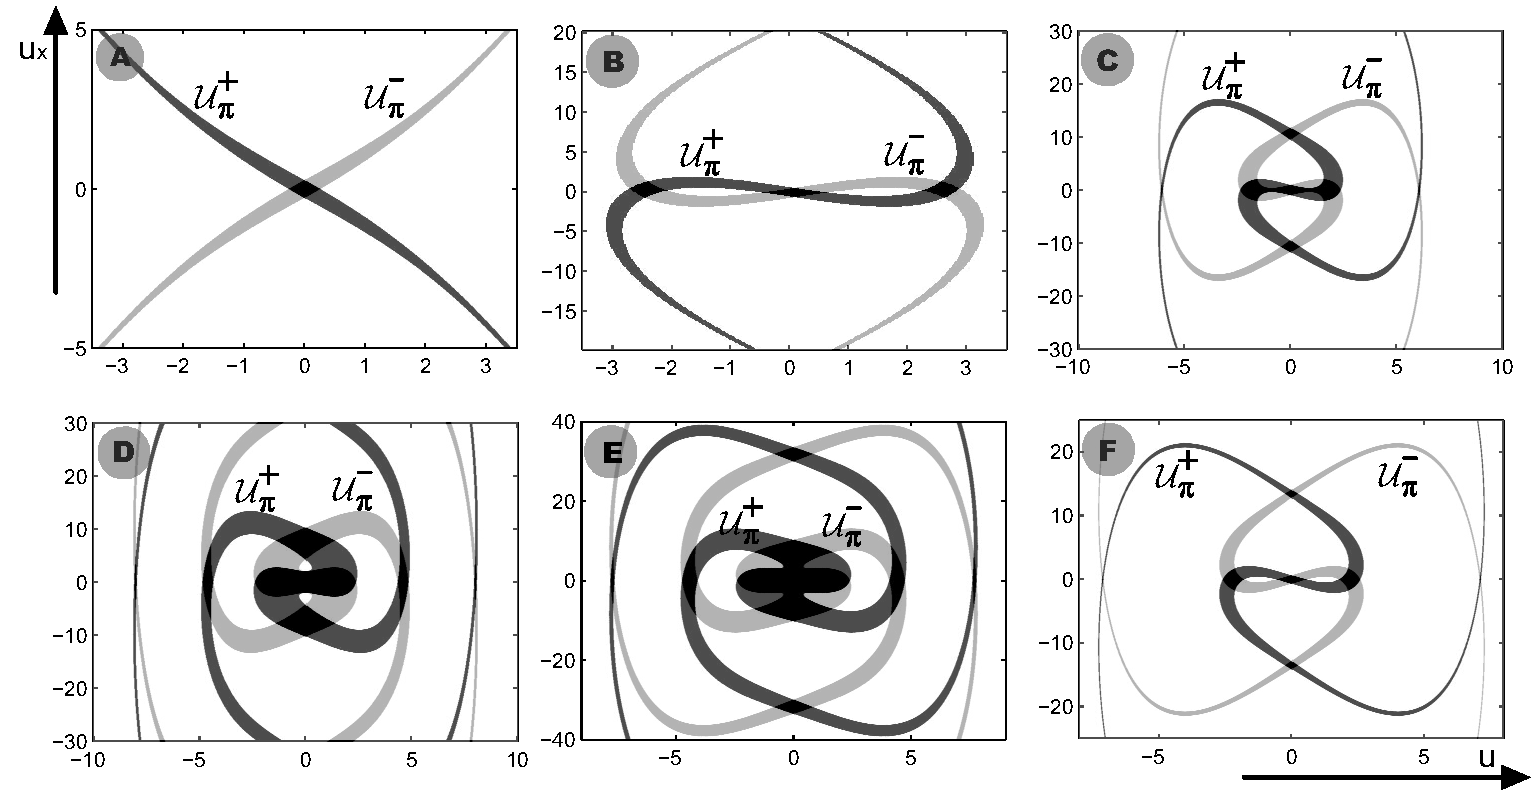
\includegraphics[width=1\textwidth]{pic/sets.pdf}
		\caption{Множества $\mathcal{U}_{\pi} = \mathcal{U}_{\pi}^+ \cap \mathcal{U}_{\pi}^-$ для различных значений $\omega$, $\alpha$.}
		\label{pic:sets}
	\end{figure}
\end{frame}

% ************
% * SLIDE 09 *
% ************
\begin{frame}
	\frametitle{Классификация}
	\framesubtitle{Построение алфавита: $\omega = -1$, $\alpha = -0.1$}
	\begin{figure}
		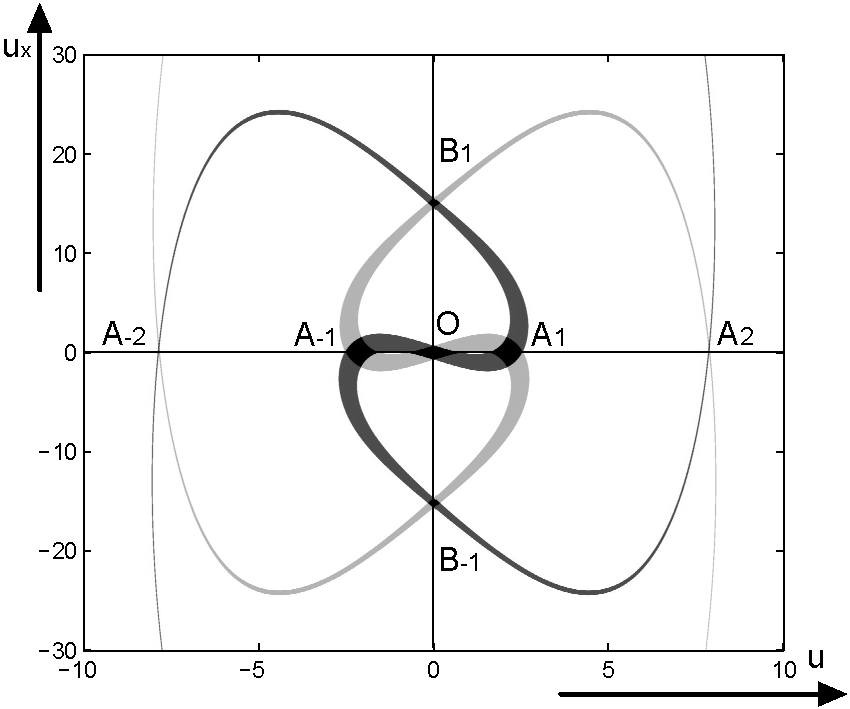
\includegraphics[width=0.75\textwidth]{pic/alphabet.pdf}
		\caption{Спиралевидная структура $\mathcal{U}_{\pi}^{\pm}$ $\Rightarrow$ бесконечный алфавит.}
		\label{pic:alphabet}
	\end{figure}
\end{frame}

% ************
% * SLIDE 10 *
% ************
\begin{frame}
	\frametitle{Классификация}
	\framesubtitle{Кодировка решений}
	
	\begin{figure}
		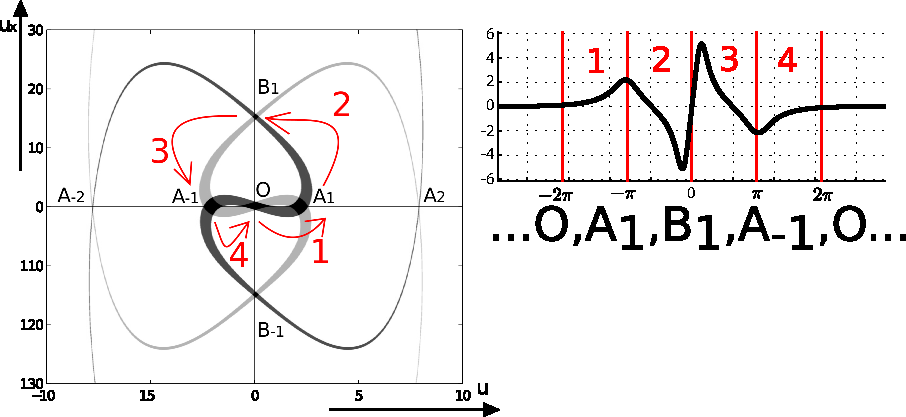
\includegraphics[width=1\textwidth]{pic/coding.pdf}
		\caption{Пример построение кода для заданного решения.}
		\label{pic:coding}
	\end{figure}
\end{frame}

% ************
% * SLIDE 11 *
% ************
\begin{frame}
	\frametitle{Классификация}
	\framesubtitle{Взаимно однозначное соответствие}
	
	Когда соответствие $\Sigma$ является взаимно однозначным?\footnotemark[3]
	\begin{enumerate}
		\item Множество $\mathcal{U}_L$ состоит из непересекающихся {\it островов}: $\mathcal{U}_L = \bigcup_{i \in S} D_i$.
		\item $\mathcal{P} D_i \cap D_j$, $\mathcal{P} D_i \cap D_j$ непусты; действие $\mathcal{P}$ на кривые внутри $D_i$ сохраняет свойства монотонности.
		\item $\Delta_0 = \mathcal{U}_L$, \quad $\Delta_{n + 1}^+ = \mathcal{P} \Delta_n^+ \cap \Delta_0$, \quad $\Delta_{n + 1}^- = \mathcal{P}^{-1} \Delta_n^- \cap \Delta_0$,\begin{center}
				$\lim \limits_{n \to \infty} \mu( \Delta_n^{\pm} ) = 0$.
			\end{center} 
	\end{enumerate}
	
	% Here could be some pictures, which clarify dynamics of the Poincare map on the phase plane.
	% Some h, v - strips could be depicted here.
	\begin{figure}
		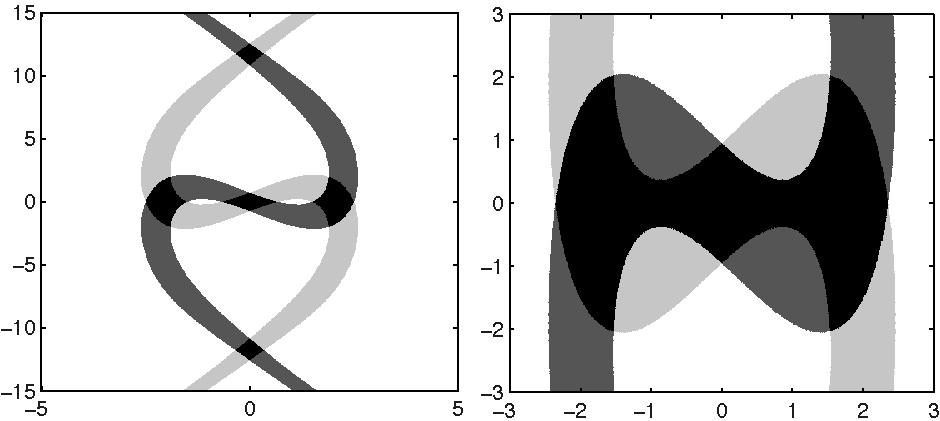
\includegraphics[width=0.5\textwidth]{pic/islands.pdf}
		\caption{Пример островного и не островного множества $\mathcal{U}_{L}$.}
		\label{pic:coding}
	\end{figure}
	
	\footnotetext[3]{\footnotesize{G. L. Alfimov, A. I. Avramenko, Physica D 254, 29 (2013)}}
\end{frame}

% ************
% * SLIDE 12 *
% ************
\begin{frame}	
	\begin{figure}
		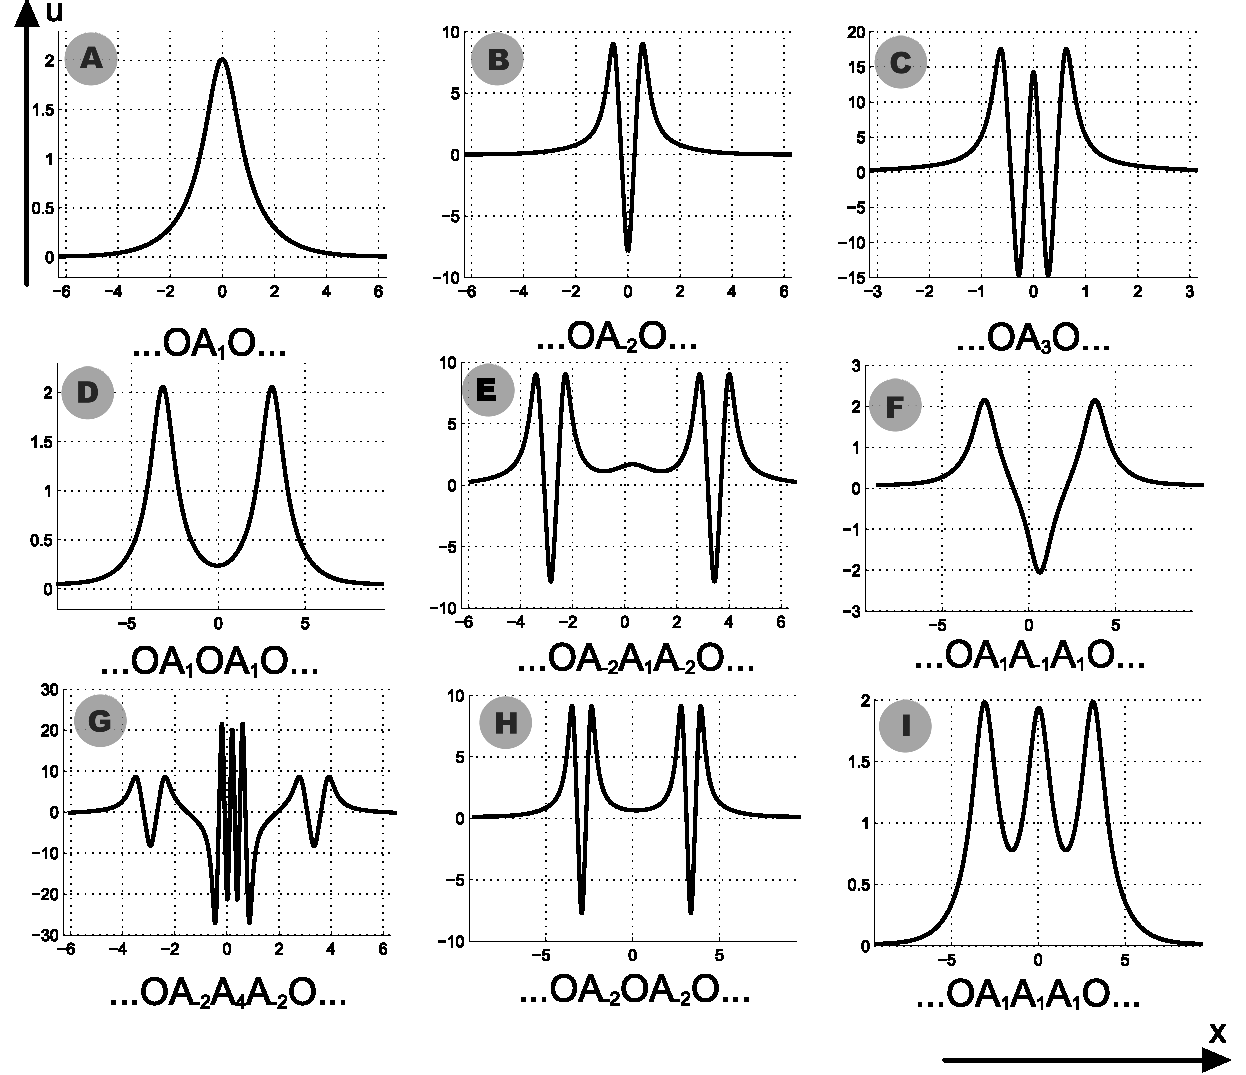
\includegraphics[width=0.9\textwidth]{pic/classification.pdf}
		\caption{Решения и их коды при $\omega = -1$, $\alpha = -0.1$.}
		\label{pic:classification}
	\end{figure}
\end{frame}

% ************
% * SLIDE 13 *
% ************
\begin{frame}
	\frametitle{Устойчивость}
	\framesubtitle{Аппарат\footnotemark[4]}
	
	Исходное уравнение:
	\begin{equation}
		i \Psi_t + \Psi_{xx} + F(|\Psi|^2, x) \Psi = 0.
		\label{eq:stability}
	\end{equation}

	Малые возмущения стационарного решения:
	\begin{equation}
		\Psi(t, x) = (u(x) + \widetilde{R}(t, x)) e^{-i \omega t}, \quad \widetilde{R} \ll 1.
		\label{eq:perturbation}
	\end{equation}
	
	Ищем решение в виде:
	\begin{equation}
		\widetilde{R}(t, x) = (a(x) + b(x)) e^{\lambda t} + (a^*(x) - b^*(x)) e^{\lambda^* t}.
		\label{eq:ansatz}
	\end{equation}
	
	Задача на собственные значения:
	\begin{equation}
		i \begin{pmatrix} 0 & \mathcal{L}_0 \\ \mathcal{L}_1 & 0 \end{pmatrix} \begin{pmatrix} a \\ b \end{pmatrix} = \lambda \begin{pmatrix} a \\ b \end{pmatrix};
		\label{eq:eigenvalues}
	\end{equation}
	\begin{eqnarray}
		&& \mathcal{L}_0 = \partial_{xx} + \omega + F(u^2, x); \\
		&& \mathcal{L}_1 = \partial_{xx} + \omega + F(u^2, x) + 2u^2 F_{|\Psi|^2}(u^2, x).
	\end{eqnarray}
	
	\footnotetext[4]{\footnotesize{Jianke Yang, Nonlinear Waves in Integrable and Nonintegrable Systems // Society of Industrial and Applied Mathematics (2010)}}
\end{frame}

% ************
% * SLIDE 14 *
% ************
\begin{frame}
	\frametitle{Устойчивость}
	\framesubtitle{Метод коллокаций Фурье}
	
	Рассматриваем локализованное решение на отрезке: $[-\frac{M}{2}; \frac{M}{2}]$.
	
	Ищем решение задачи \eqref{eq:eigenvalues} в виде разложений в ряды Фурье:
	\begin{equation}
		a(x) = \sum \limits_{n \in \mathbb{Z}} a_n e^{i \frac{2 \pi n}{M} x}, \quad b(x) = \sum \limits_{n \in \mathbb{Z}} b_n e^{i \frac{2 \pi n}{M} x}.
		\label{eq:solutions_expansions}
	\end{equation}
	
	Соответствующие представления для операторов $\mathcal{L}_0$, $\mathcal{L}_1$:
	\begin{equation}
		\mathcal{L}_0 = \partial_{xx} + \sum \limits_{n \in \mathbb{Z}} c_n^{(0)} e^{i \frac{2 \pi n}{M} x}, \quad \mathcal{L}_1 = \partial_{xx} + \sum \limits_{n \in \mathbb{Z}} c_n^{(1)} e^{i \frac{2 \pi n}{M} x}.
		\label{eq:operators_expansions}
	\end{equation}
	
	Подставляя \eqref{eq:solutions_expansions}, \eqref{eq:operators_expansions} в \eqref{eq:eigenvalues}, получаем систему линейных уравнений:
	\begin{equation}
		\begin{cases}
			-i \lambda a_k = -b_k (k k_0)^2 + \sum \limits_{n \in \mathbb{Z}} c_n^{(0)} b_{k - n} \\
			-i \lambda b_k = i a_k (k k_0)^2 + i \sum \limits_{n \in \mathbb{Z}} c_n^{(1)} a_{k - n} \\
		\end{cases}, \quad k \in \mathbb{Z}.
		\label{eq:system}
	\end{equation}
	
	Ограничим количество гармоник Фурье: $k \in [-K; K]$ $\Rightarrow$ задача на собственные значения оператора конечной размерности.
\end{frame}

% ************
% * SLIDE ?? *
% ************
%\begin{frame}
%	\frametitle{Устойчивость}
%	\framesubtitle{Недостатки подхода}
%	Осцилляторная неустойчивость, функция Эванса.
%\end{frame}

% ************
% * SLIDE 15 *
% ************
\begin{frame}
	\frametitle{Устойчивость}
	\framesubtitle{Тест}
	
	\begin{enumerate}
		\item[(A)] Решение $|\Psi(t, x)|$ {\it {\color{forestgreen} линейной устойчиво}}: весь спектр $\{ \lambda_i \}$ является мнимым.
		\item[(B)] Решение $|\Psi(t, x)|$ {\it {\color{fireenginered} экспоненциально неустойчиво}}: $\exists$ пара действительных собственных значений $\pm \lambda$.
		\item[(C)] Решение $|\Psi(t, x)|$ {\it {\color{fireenginered} осцилляторно неустойчиво}}: $\exists$ четверка комплексных собственных значений $\pm \lambda$, $\pm \lambda^*$.
	\end{enumerate}
	
	\begin{figure}
		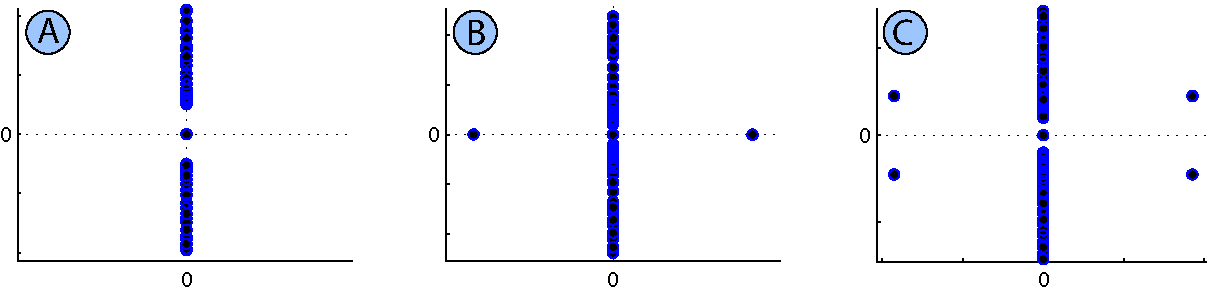
\includegraphics[width=0.8\textwidth]{pic/test.pdf}
		\caption{Примеры спектров для различных типов устойчивости.}
		\label{pic:test}
	\end{figure}
	
	Далее представлены результаты для:
	$$F(|\Psi|^2, x) = (\alpha + \cos 2x) |\Psi|^2.$$
\end{frame}

% ************
% * SLIDE 16 *
% ************
\begin{frame}
	\frametitle{Устойчивость}
	\framesubtitle{Примеры: фундаментальное решение}
	
	\begin{figure}
		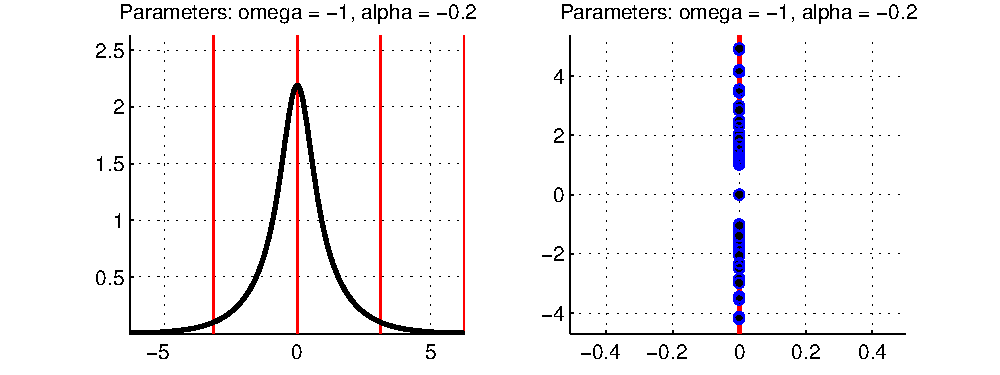
\includegraphics[width=1\textwidth]{pic/example_1.pdf}
		\caption{Фундаментальное решение $\dots O A_1 O \dots$, {\it \color{forestgreen}{линейно устойчиво}}.}
		\label{pic:example_1}
	\end{figure}
\end{frame}

% ************
% * SLIDE 17 *
% ************
\begin{frame}
	\frametitle{Устойчивость}
	\framesubtitle{Примеры: дипольное решение\footnotemark[5]}
	
	\begin{figure}
		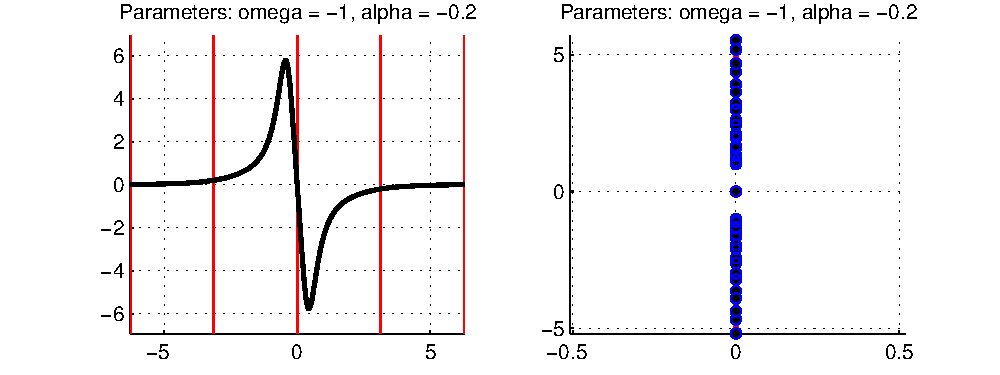
\includegraphics[width=1\textwidth]{pic/example_2.pdf}
		\caption{Дипольное решение $\dots O B_{-1} O \dots$, {\it \color{forestgreen}{линейно устойчиво}}.}
		\label{pic:example_2}
	\end{figure}
	
	\footnotetext[5]{\footnotesize{M. E. Lebedev, G. L. Alfimov, B. A. Malomed // Chaos: An Interdisciplinary Journal of Nonlinear Science 26 (7), 073110 (2016)}}
\end{frame}

% ************
% * SLIDE 18 *
% ************
\begin{frame}
	\frametitle{Устойчивость}
	\framesubtitle{Примеры}
	
	\begin{figure}
		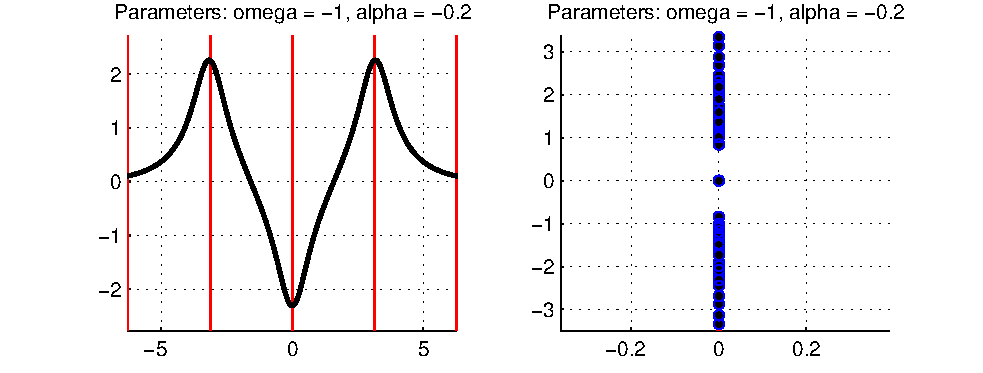
\includegraphics[width=1\textwidth]{pic/example_3.pdf}
		\caption{Решение $\dots O A_1 A_{-1} A_1 O \dots$, {\it \color{forestgreen}{линейно устойчиво}}.}
		\label{pic:example_3}
	\end{figure}
\end{frame}

% ************
% * SLIDE 19 *
% ************
\begin{frame}
	\frametitle{Устойчивость}
	\framesubtitle{Примеры}
	
	\begin{figure}
		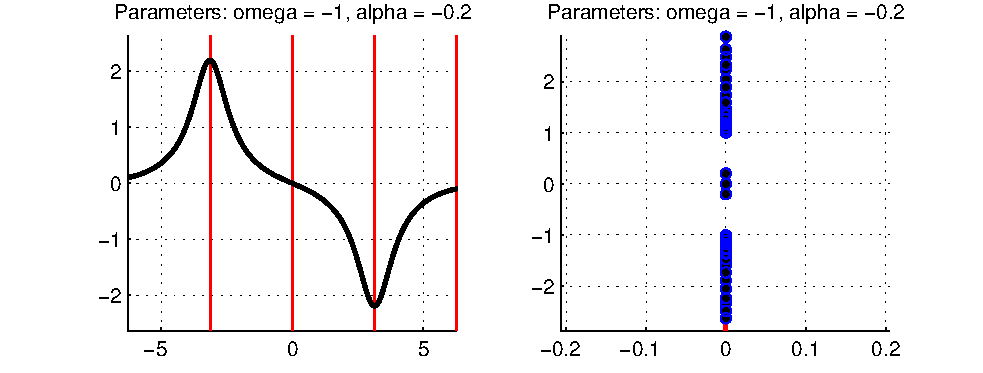
\includegraphics[width=1\textwidth]{pic/example_4.pdf}
		\caption{Решение $\dots O A_1 O A_{-1} O \dots$, {\it \color{forestgreen}{линейно устойчиво}}.}
		\label{pic:example_4}
	\end{figure}
\end{frame}

% ************
% * SLIDE 20 *
% ************
\begin{frame}
	\frametitle{Устойчивость}
	\framesubtitle{Примеры}
	
	\begin{figure}
		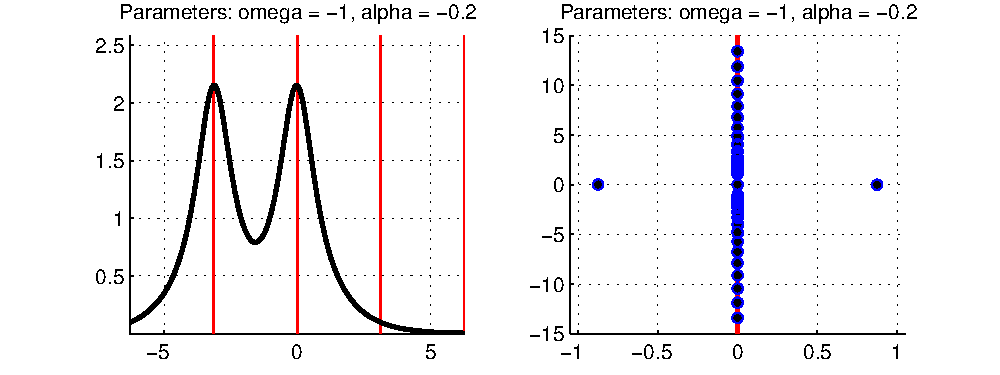
\includegraphics[width=1\textwidth]{pic/example_5.pdf}
		\caption{Решение $\dots O A_1 A_1 O \dots$, {\it \color{fireenginered}{экспоненциально неустойчиво}}.}
		\label{pic:example_5}
	\end{figure}
\end{frame}

% ************
% * SLIDE 21 *
% ************
\begin{frame}
	\frametitle{Устойчивость}
	\framesubtitle{Примеры}
	
	\begin{figure}
		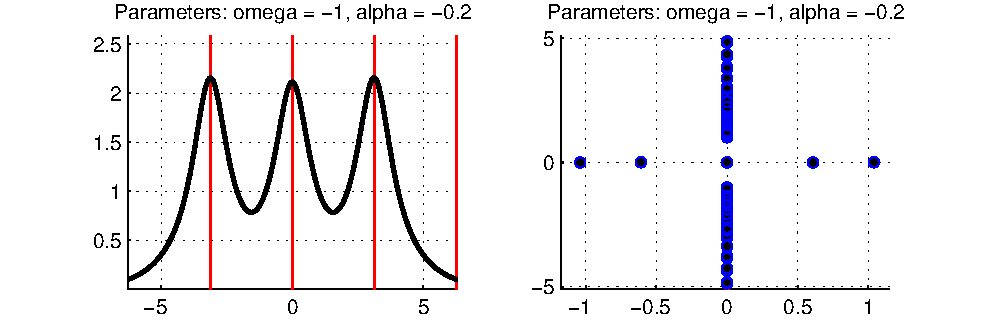
\includegraphics[width=1\textwidth]{pic/example_6.pdf}
		\caption{Решение: $\dots O A_1 A_1 A_1 O \dots$, {\it \color{fireenginered}{экспоненциально неустойчиво}}.}
		\label{pic:example_6}
	\end{figure}
\end{frame}

% ************
% * SLIDE 22 *
% ************
\begin{frame}
	\frametitle{Устойчивость}
	\framesubtitle{Примеры}
	
	\begin{figure}
		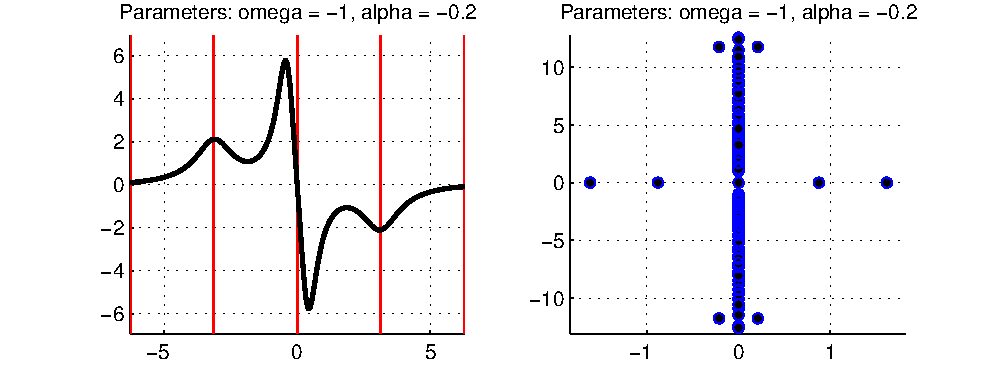
\includegraphics[width=1\textwidth]{pic/example_7.pdf}
		\caption{Решение: $\dots O A_1 B_{-1} A_{-1} O \dots$, {\it \color{fireenginered}{экспоненциально неустойчиво}}.}
		\label{pic:example_7}
	\end{figure}
\end{frame}

% ************
% * SLIDE 23 *
% ************
\begin{frame}
	\frametitle{Устойчивость}
	\framesubtitle{Примеры}
	
	\begin{figure}
		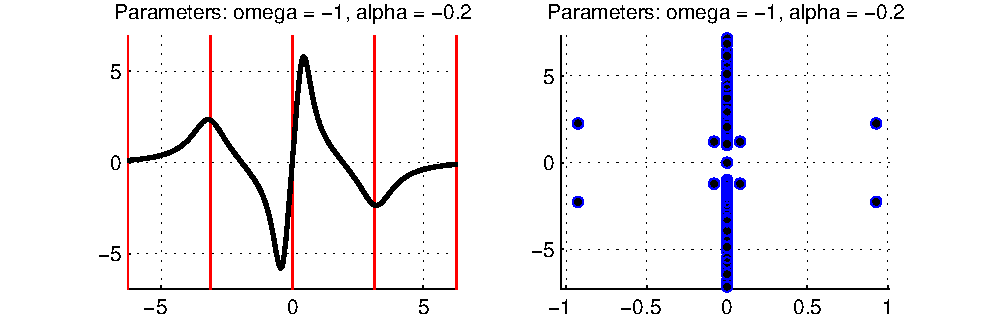
\includegraphics[width=1\textwidth]{pic/example_8.pdf}
		\caption{Решение: $\dots O A_1 B_1 A_{-1} O \dots$, {\it \color{fireenginered}{осцилляторно неустойчиво}}.}
		\label{pic:example_8}
	\end{figure}
\end{frame}

% ************
% * SLIDE 24 *
% ************
\begin{frame}
	\frametitle{Устойчивость}
	\framesubtitle{Результаты\footnotemark[5]}
	
	\begin{equation}
		i \Psi_t + \Psi_{xx} + (\alpha + \cos 2x) |\Psi|^2 \Psi = 0
		\label{eq:results}	
	\end{equation}
	
	\begin{itemize}
		\item Множество стационарных решений уравнения \eqref{eq:results} чрезвычайно богато.
		\item Большинство стационарных решений оказываются неустойчивы; исключение составляют:
			\begin{enumerate}
				\item[1.] Фундаментальное решение: $\dots O A_{\pm 1} O \dots$.
				\item[2.] Дипольное решение: $\dots O B_{\pm 1} O \dots$ ({\bf {\color{red} new}}).
				\item[3.] Некоторые комбинации {\color{ceruleanblue} (1)} и {\color{ceruleanblue} (2)}: $\dots O A_1 A_{-1} A_1 O \dots$, $\dots O A_1 O A_{-1} O \dots$.
			\end{enumerate}
	\end{itemize}
	
	\footnotetext[5]{\footnotesize{M. E. Lebedev, G. L. Alfimov, B. A. Malomed // Chaos: An Interdisciplinary Journal of Nonlinear Science 26 (7), 073110 (2016)}}
\end{frame}

% ************
% * SLIDE 25 *
% ************
\begin{frame}
	\frametitle{Устойчивость}
	\framesubtitle{Расчёт эволюции}
	
	Для расчёта используем консервативную разностную схему Трофимова--Пескова\footnotemark[6].
	Она сохраняет два интеграла:
	\begin{equation}
		N(t) = \int |\Psi(t, x)|^2 dx; \quad
		E(t) = \dfrac{1}{2} \int \Psi^*(t, x) \widehat{H} \Psi(t, x) dx
	\end{equation}

	Для подавления эффекта отражения излучения от краев области интегрирования при расчете, в схему добавлен {\it {\color{ceruleanblue} поглощающий слой}}. 
	
	\footnotetext[6]{\footnotesize{V. A. Trofimov, N. V. Peskov // Mathematical Modelling and Analysis, Volume 14 Number 1, 2009, pages 109-126}}
\end{frame}

% ************
% * SLIDE 26 *
% ************
\begin{frame}
	\frametitle{Устойчивость}
	\framesubtitle{Расчёт эволюции: дипольное решение}
	
	\begin{figure}
		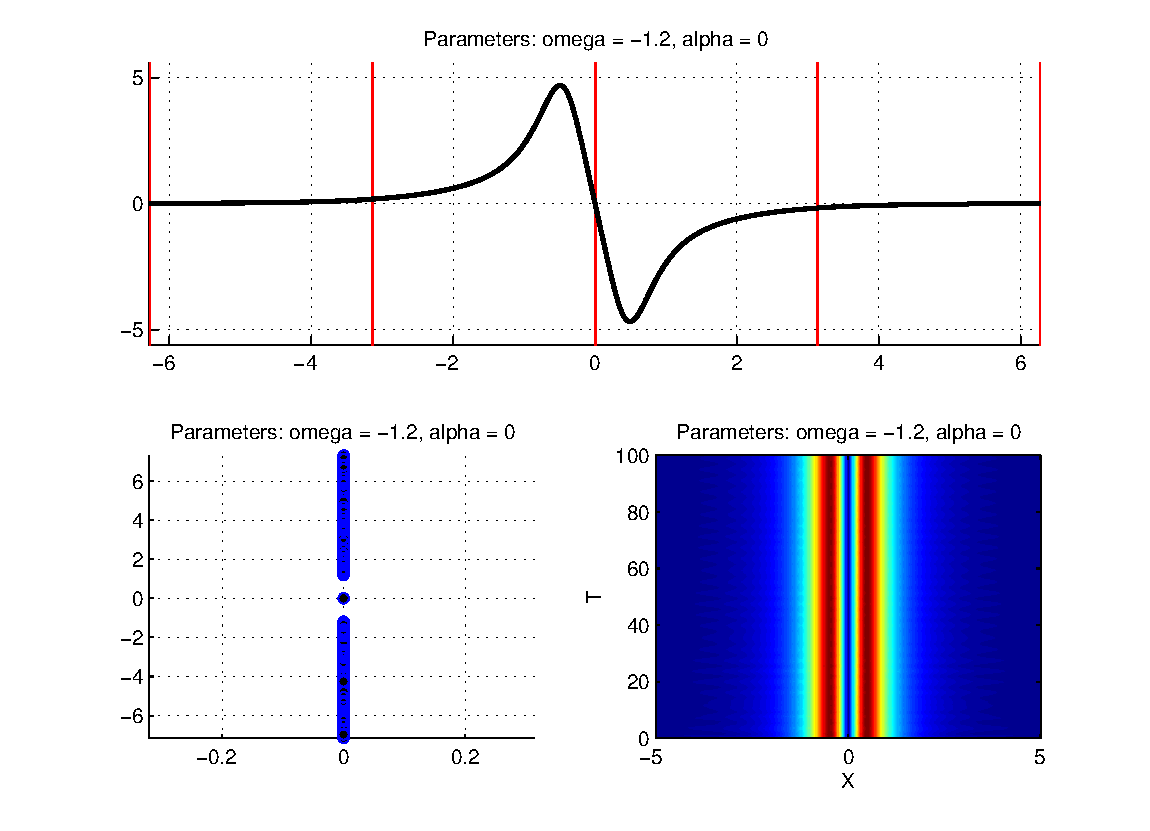
\includegraphics[width=0.85\textwidth]{pic/dipole_solution_stable.pdf}
		\caption{Устойчивое дипольное решение.}
		\label{pic:dipole_solution_stable}
	\end{figure}
\end{frame}

% ************
% * SLIDE 27 *
% ************
\begin{frame}
	\frametitle{Устойчивость}
	\framesubtitle{Расчёт эволюции: дипольное решение}
	
	\begin{figure}
		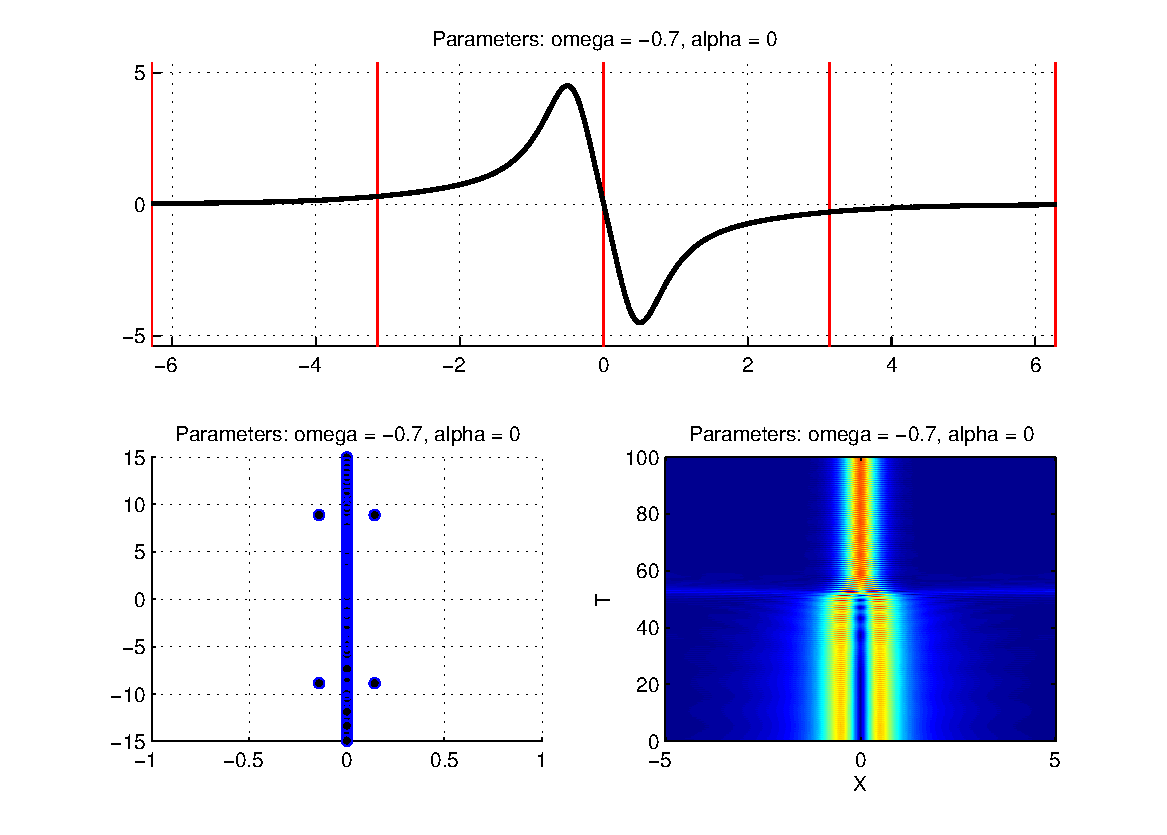
\includegraphics[width=0.85\textwidth]{pic/dipole_solution_unstable.pdf}
		\caption{Неустойчивое дипольное решение.}
		\label{pic:dipole_solution_unstable}
	\end{figure}
\end{frame}

% ************
% * SLIDE 28 *
% ************
\begin{frame}
	\frametitle{Классическая потенциальная яма}
	\framesubtitle{Простейший нелинейный потенциал\footnotemark[7]}
	
	\begin{equation}
		i \Psi_t + \Psi_{xx} - x^2 \Psi \pm |\Psi|^2 \Psi = 0.
	\end{equation}
	
	Все локализованные решения имеют {\it \uwave{линейный аналог}}.
	
	\begin{figure}
		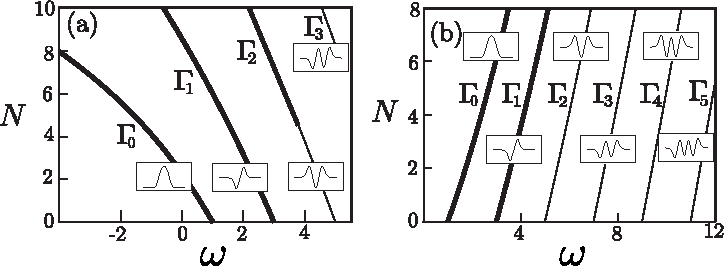
\includegraphics[width=0.9\textwidth]{pic/solution_branches_simple.pdf}
		\caption{Ветви различных локализованных решений и их устойчивость для случаев {\color{ceruleanblue} (a)} $P(x) \equiv +1$; {\color{ceruleanblue} (b)} $P(x) \equiv -1$.}
		\label{pic:branches_simple}
	\end{figure}
	
	\footnotetext[7]{\footnotesize{D. A. Zezyulin, G. L. Alfimov, V. V. Konotop and V. M. P\'erez-Garcia // Phys. Rev. A {\bf 76}, 013621 (2007)}}
\end{frame}

% ************
% * SLIDE 28 *
% ************
\begin{frame}
	\frametitle{Классическая потенциальная яма}
	\framesubtitle{Периодический нелинейный потенциал с ненулевой средней}
	
	\begin{equation}
		i \Psi_t + \Psi_{xx} - x^2 \Psi + (1 + \beta \cos \Omega x) |\Psi|^2 \Psi = 0.
	\end{equation}

	Появляются решения, {\it не имеющие линейного аналога}.

	\begin{figure}
		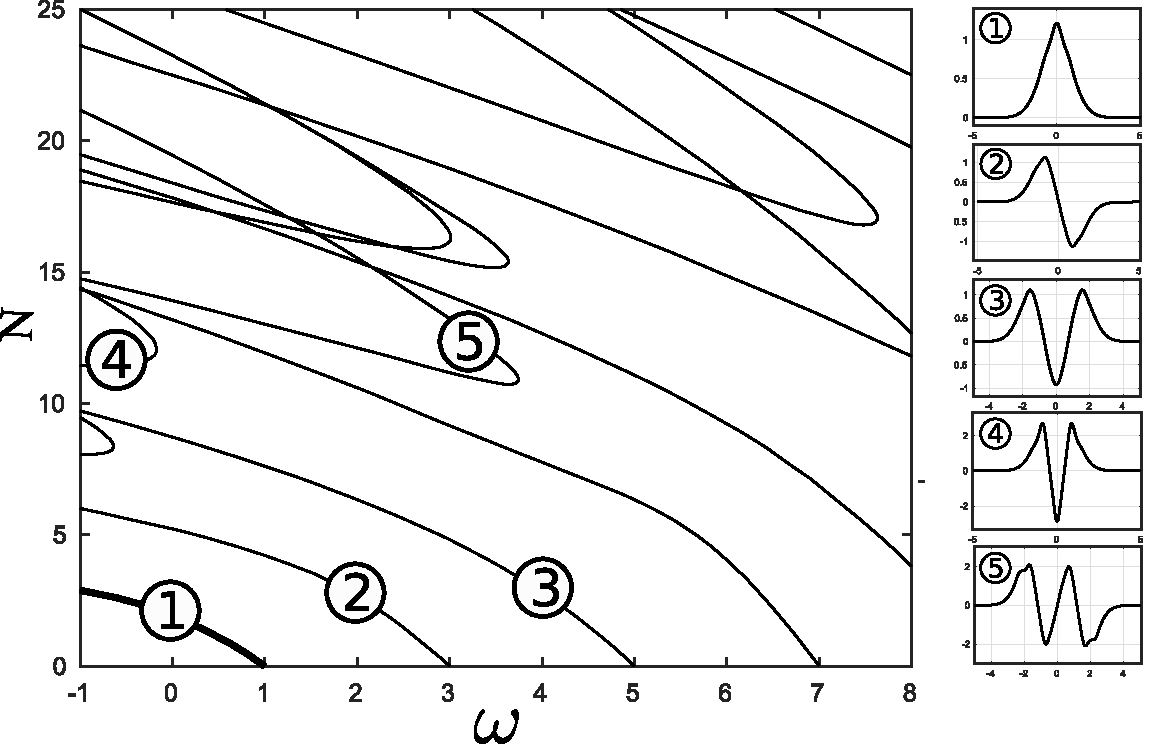
\includegraphics[width=0.7\textwidth]{pic/solution_branches_nonzero_mean.pdf}
		\caption{Ветви различных локализованный решений и их устойчивость для $\beta = 2$, $\Omega = 8$.}
		\label{pic:branches_nonzero_mean}
	\end{figure}	
	
\end{frame}

% ************
% * SLIDE 29 *
% ************
\begin{frame}
	\frametitle{Классическая потенциальная яма}
	\framesubtitle{Периодический нелинейный потенциал с нулевой средней}
	
	\begin{equation}
		i \Psi_t + \Psi_{xx} - x^2 \Psi + \cos \Omega x |\Psi|^2 \Psi = 0.
	\end{equation}

	Ветвь решения {\color{ceruleanblue} (1)} устойчива при $\omega \approx 5$.

	\begin{figure}
		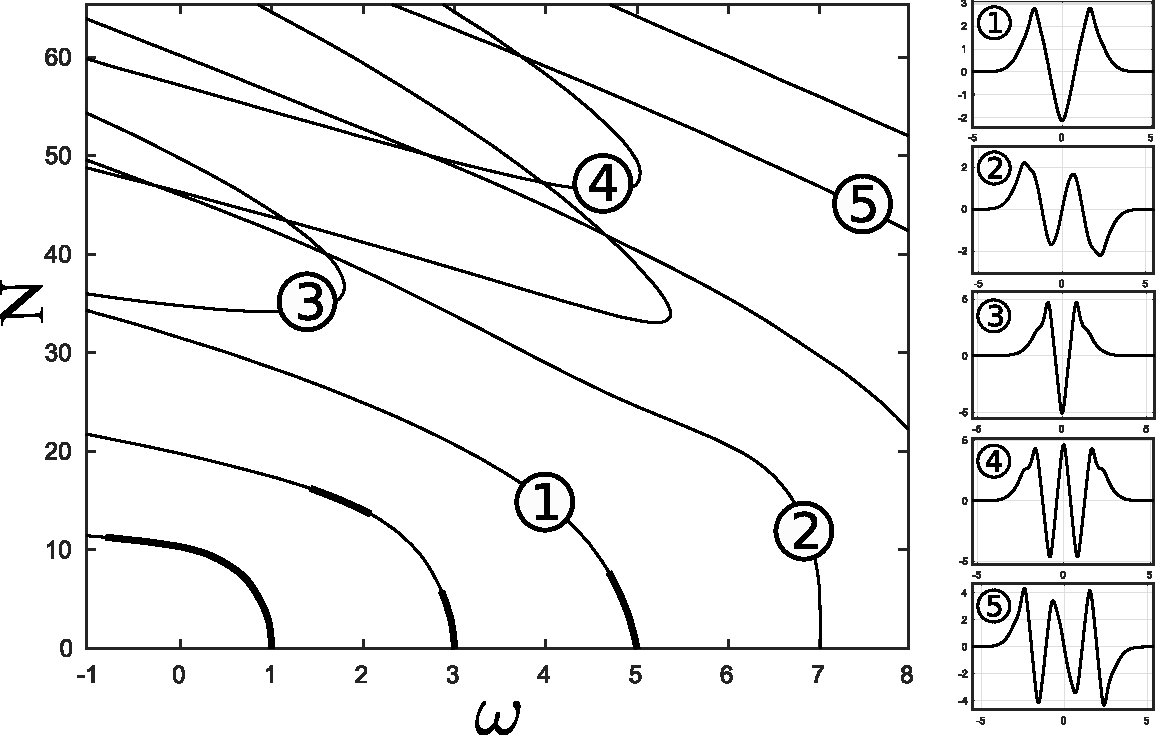
\includegraphics[width=0.7\textwidth]{pic/solution_branches_zero_mean.pdf}
		\caption{Ветви различных локализованный решений и их устойчивость для $\Omega = 8$.}
		\label{pic:branches_zero_mean}
	\end{figure}	
	
\end{frame}

% ************
% * SLIDE 30 *
% ************
\begin{frame}
	\frametitle{Предельный переход $\Omega \to +\infty$}
	\framesubtitle{Периодический нелинейный потенциал с ненулевой средней}
	
	\begin{figure}
		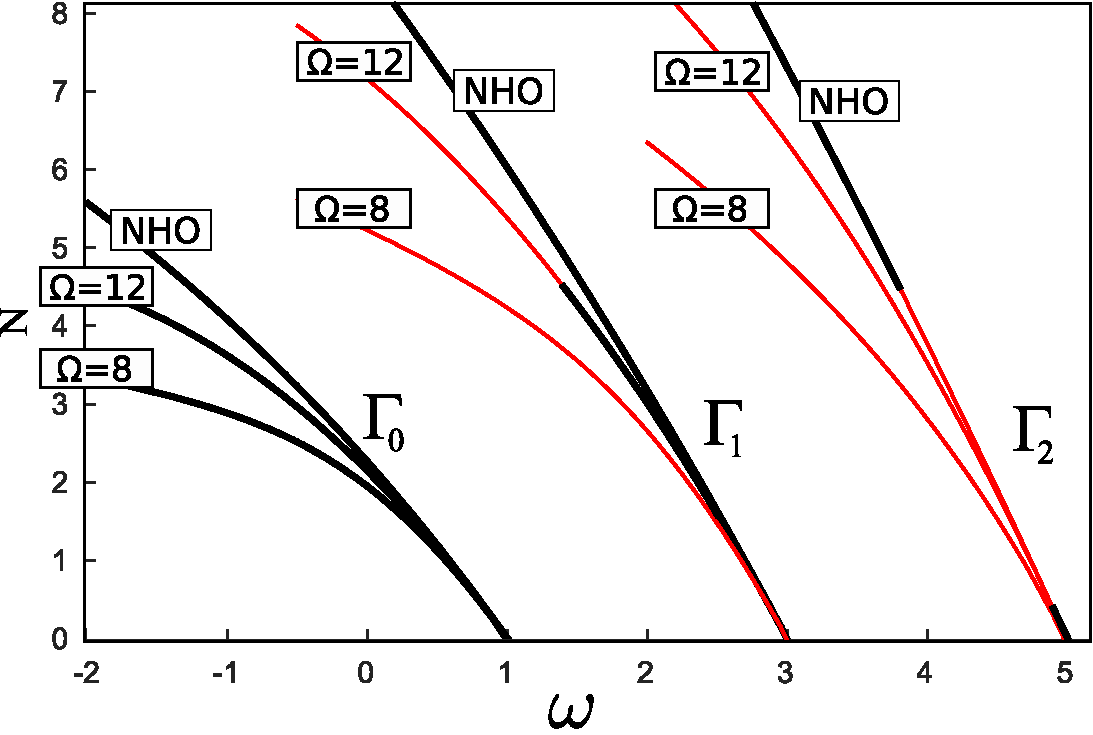
\includegraphics[width=0.85\textwidth]{pic/nonlinear_oscillator_limit.pdf}
		\caption{Переход к нелинейному гармоническому осциллятору при $\Omega \to +\infty$ для $P(x) = 1 + \cos \Omega x$.}
		\label{pic:nonlinear_limit}
	\end{figure}	
\end{frame}

% ************
% * SLIDE 31 *
% ************
\begin{frame}
	\frametitle{Предельный переход $\Omega \to +\infty$}
	\framesubtitle{Периодический нелинейный потенциал с нулевой средней}
	
	\begin{figure}
		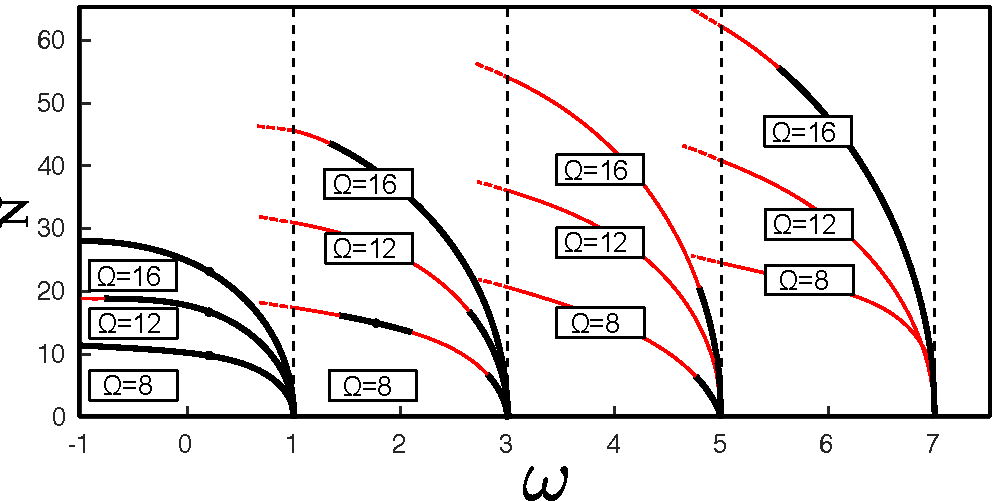
\includegraphics[width=0.85\textwidth]{pic/linear_oscillator_limit.pdf}
		\caption{Переход к линейному гармоническому осциллятору при $\Omega \to +\infty$ для $P(x) = \cos \Omega x$.}
		\label{pic:linear_limit}
	\end{figure}
\end{frame}

% ************
% * SLIDE 32 *
% ************
\begin{frame}
	\frametitle{Потеря устойчивости решений с линейным аналогом}
	
	\begin{figure}
		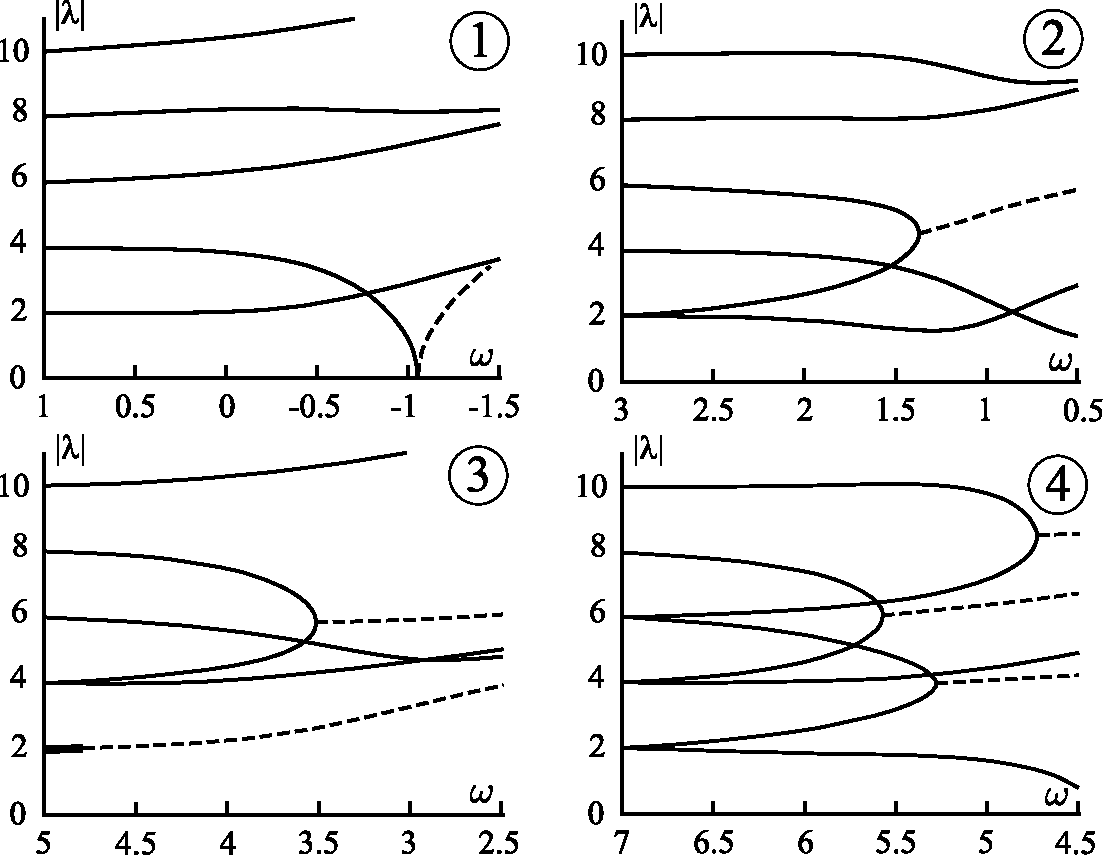
\includegraphics[width=0.85\textwidth]{pic/stability_loss.pdf}
		\caption{Сценарии потери устойчивости первых четырёх ветвей  решений с линейным аналогом для $P(x) = \cos 16 x$.}
		\label{pic:stability_loss}
	\end{figure}
\end{frame}

% ************
% * SLIDE ?? *
% ************
%\begin{frame}
%	\frametitle{Сценарий потери устойчивости}
%	\framesubtitle{Асимптотическое приближение}
%\end{frame}

% ************
% * SLIDE 33 *
% ************
\begin{frame}
	\frametitle{Классическая потенциальная яма}
	\framesubtitle{Расчёт эволюции}
	
	\begin{figure}
		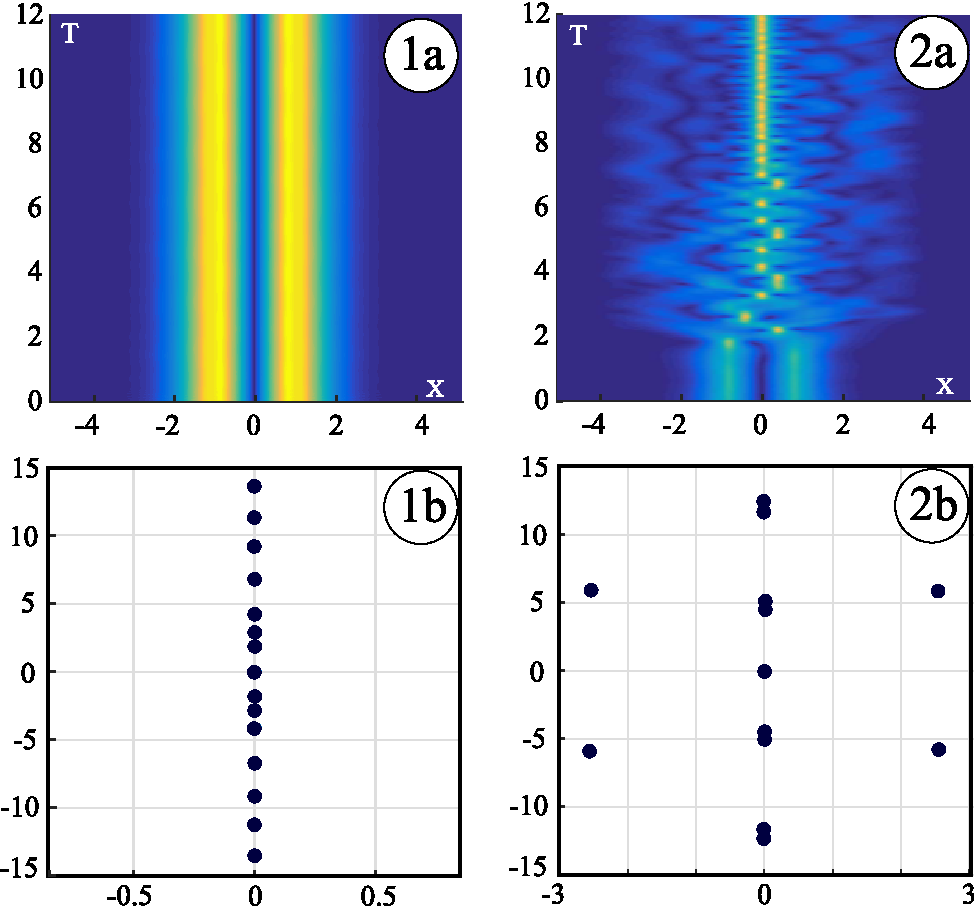
\includegraphics[width=0.7\textwidth]{pic/evolution.pdf}
		\caption{Решение $\Gamma_1$ при $P(x) = \cos 16 x$ для {\color{ceruleanblue} (1)} $\omega = 2$ и {\color{ceruleanblue} (2)} $\omega = 0$.}
		\label{pic:evolution}
	\end{figure}
\end{frame}

% ************
% * SLIDE 34 *
% ************
\begin{frame}
	\frametitle{Классическая потенциальная яма}
	\framesubtitle{Результаты\footnotemark[7]}
	
	\begin{itemize}
		\item Присутствие периодического нелинейного потенциала приводит к появлению локализованных решений без линейного аналога.
		\item В предельном случае $\Omega \to +\infty$ задача приближается к линейному или нелинейному гармоническому осциллятору.
		\item Сценарий потери устойчивости для решений с линейным аналогом ({\it {\color{ceruleanblue} исследован асимптотически}}):
		\begin{enumerate}
			\item При $P(x) = 0$ некоторые $\lambda_i$ удвоены.
			\item Удвоенные $\lambda_i$ расщепляются под действием возмущения $P(x) \neq 0$.
			\item При расщеплении могут образовывать $\lambda_i$ с ненулевой действительной частью.
		\end{enumerate}
	\end{itemize}
	
	\footnotetext[7]{\footnotesize{G. L. Alfimov, L. A. Gegel, M. E. Lebedev, B. A. Malomed, D. A. Zezyulin // Communications in Nonlinear Science and Numerical Simulation {\bf 66}, 194-207 (2019).}}
\end{frame}

% ************
% * SLIDE XX *
% ************
%\begin{frame}
%	\frametitle{Содержание}
%	\tableofcontents
%\end{frame}

% ************
% * SLIDE YY *
% ************
\begin{frame}
	\begin{center}
		Спасибо за внимание\ex
	\end{center}
\end{frame}

\end{document} 